\section{Image Segmentation\buch{Ch. 10}\buchSeite{689-794}}
\paragraph{Preliminaries}
\begin{itemize}
\item Separate the image into different parts, ie. regions or objects
\item It is a difficult but important task
\item Often a scene can be designed that the segmentation task is simplified
\item Segmentation is based on some property of the scene
\begin{itemize}
\item Intensity discontinuity
\item Intensity similarity
\item More Complex properties:
\begin{itemize}
\item Motion
\item Texture
\item Shape
\item Color
\item etc.
\end{itemize}
\end{itemize}
\end{itemize}

\subsection{Fundamentals\buchSeite{690}}
\begin{figure}[!h]
\begin{subfigure}[b]{0.48\textwidth}
\begin{enumerate}[label={\alph*)}]
\item $\bigcup\limits_{i=1}^{n}R_i=R$
\item $R_i$ is a connected set, $i=1,2,...,n$
\item $R_i\bigcap R_j = 0$ for all $i$ and $j, i\neq j$
\item $Q(R_i)=$TRUE for $i=1,2,...n$
\item $Q(R_i\bigcup R_j)=$FALSE for any adjacent Regions $R_i$ and $R_j$
\end{enumerate}
\end{subfigure}
\begin{subfigure}[b]{0.48\textwidth}
\begin{itemize}
\item The entire spatial region that is occupied by an image is called $R$
\item Image segmentation is the task of partitioning R into sub-regions $R_i$
\item $Q()$ is a measure of similarity of a particular property
\item d) must be true, since this defines the region
\item e) must be false, since otherwise, the regions should have been merged
\end{itemize}
\end{subfigure}
\end{figure}

Focus on the intenxity values
\begin{itemize}
\item there are discontinuities, then a new region starts.
\item If the intensity does not vary much, then this is one region.
\end{itemize}

\subsection{Point, line and edge detection\buchSeite{692}}

When the intensity changes abruptly in a local neighborhood, this indicates an edge. It can be a simple point or a line.

\subsubsection{Background\buchSeite{692}}

Abrupt local changes can be detected using derivatives.\\
First order derivative
\[
	\frac{\partial f}{\partial x} = f'(x)=f(x+1)-f(x)
\]
The second order derivative
\[
	\frac{\partial^2f}{\partial x^2}=\frac{\partial f'(x)}{\partial x}=f''(x)=f(x+1)+f(x-1)-2f(x)
\]
This can be calculated using a spatial filter.
\[
	\begin{matrix}
	w_1, w_2, w_3\\
	w_4, w_5, w_6\\
	w_7, w_8, w_9
	\end{matrix}
\]
\begin{itemize}
\item First order in y direction $w_6=1, w_5=-1$
\item First order in x direction $w_8=1, w_5=-1$
\item Second order in y direction $w_6=1, w_4=1, w_5=-2$
\item Second order in x direction $w_8=1, w_2=1, w_5=-2$
\end{itemize}
\subsubsection{Detection of Isolated Points\buchSeite{696}}
The Laplacian combines the second derivatives in both spatial directions. This results in
\[
	\nabla^2f(x,y)=f(x+1,y)+f(x-1,y)+f(x,y+1)+f(x,y-1)-4f(x,y)
\]
It can be extended to also include the diagonal terms wich results in the following mask
\[
	\begin{matrix}
	 1 & 1 & 1\\
	 1 & -8 & 1\\
	 1 & 1 & 1
	\end{matrix}
\]
The Laplacian is isotropic with respect to $0^\circ, 45^\circ, 90^\circ \text{ and } 135^\circ$. 

\subsubsection{Line Detection\buchSeite{697}}
Often, a line of a known direction should be detected. We use special masks for that particular direction
\begin{figure}[h]
	\centering
	\begin{subfigure}[b]{0.2\textwidth}
		\centering
		\begin{tikzpicture}
			\matrix[3x3mask]{
				-1 & -1 & -1 \\%
		    	2  & 2  & 2 \\%
				-1 & -1 & -1\\};
		\end{tikzpicture}
		\caption{Horizontal}
	\end{subfigure}
	\begin{subfigure}[b]{0.2\textwidth}
		\centering
		\begin{tikzpicture}
			\matrix[3x3mask]{
				2  & -1 & -1 \\%
				-1 & 2  & -1 \\%
				-1 & -1 & 2 \\%
			};
		\end{tikzpicture}
		\caption{$+45^\circ$}
	\end{subfigure}
	\begin{subfigure}[b]{0.2\textwidth}
		\centering
		\begin{tikzpicture}
			\matrix[3x3mask]{
				-1  & 2 & -1 \\%
				-1 & 2  & -1 \\%
				-1 & 2 & -1 \\%
				};
		\end{tikzpicture}
		\caption{Vertical}
	\end{subfigure}
	\begin{subfigure}[b]{0.2\textwidth}
		\centering
		\begin{tikzpicture}
			\matrix[3x3mask]{
				-1 & -1 & 2 \\%
				-1 & 2  & -1 \\%
				2  & -1 & -1 \\%
			};
		\end{tikzpicture}
		\caption{$+45^\circ$}
	\end{subfigure}
	\caption{Line detection masks}
\end{figure}


\subsubsection{Edge Models}
\begin{figure}[!h]
	\centering
	\documentclass[border=10pt]{standalone}
\usepackage{tikz}

\begin{document}
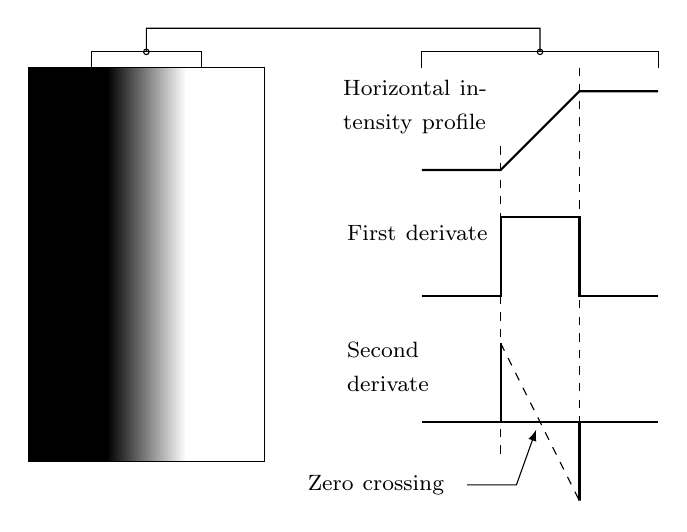
\begin{tikzpicture}
	\begin{scope}
		\fill (0,0) rectangle (1,5);
		\shade[shading angle=90, left color = black, right color = white] (1,0) rectangle (2,5);
		\fill[color=white] (2,0) rectangle (3,5);
		\draw (0,0) rectangle (3,5);
	\end{scope}
	\draw (0.8,5) -- ++(0,0.2) -- ++(1.4, 0) -- +(0,-0.2) ;
	\draw (5,5) -- ++(0,0.2) -- ++(3,0) -- +(0,-0.2);
	\draw[radius=1pt] (1.5,5.2) circle -- ++(0, 0.3) -- ++(5,0) -- ++(0,-0.3) circle;

	\begin{scope}[xshift=5cm]
		\begin{scope}[thick]
			\draw[yshift=3.7cm] (0,0) -- ++(1,0) -- ++(1,1) -- +(1,0);
			\draw[yshift=2.1cm] (0,0) -- ++(1,0) -- ++(0,1) -- ++(1,0) -- ++(0, -1) -- +(1,0);
			\draw[yshift=0.5cm] (0,0) -- ++(1,0) -- +(0,1) -- +(0,0) -- ++(1, 0) -- +(0,-1) -- +(0,0) -- +(1,0);
		\end{scope}
		\draw[dashed] (1,4) -- +(0,-4);
		\draw[dashed] (2,5) -- +(0,-5);
		\draw[yshift=0.5cm, dashed] (1,1) -- (2,-1);

		\node[text width=2cm] at (0,4.5) {\footnotesize Horizontal intensity profile};
		\node[text width=1.9cm] at (0,2.9) {\footnotesize First derivate};
		\node[text width=1.9cm] at (0,1.2) {\footnotesize Second derivate};
		\node[text width=1.9cm] (zc) at (-0.5,-0.3) {\footnotesize Zero crossing};
		\draw[-latex] (zc) -- ++(1.7, 0) -- +(0.25, 0.7);
	\end{scope}
\end{tikzpicture}
\end{document}

	\caption{Ramp Edge with intensity profile and derivates.}
\end{figure}
\subsubsection{Edge localization\buchSeite{706}}
The previously shown method generates edge points. The goal is to keep the ones which truly belong to an edge.\\
Since first order derivatives are helpful, a nice way of combining the two partial derivatives into one value is the magnitude of the gradient
\begin{equation}
	\nabla f = grad(f) = \left[\begin{array}{c} g_x \\ g_y \end{array}\right] =  \left[\displaystyle{\begin{array}{c} \frac{\partial f}{\partial x} \vspace{0.2cm}  \\ \frac{\partial f}{\partial y} \end{array}}\right] \notag
\end{equation}

The gradient (which is a vector) points into the direction of the greatest rate of change of f at the location (x,y)\\
The magnitude of the gradient vector is the value of the rate of change in that direction\\
Gradient operators:\\
\begin{figure}[h]
	\centering
	\begin{subfigure}[b]{0.2\textwidth}
		\centering
		\begin{tikzpicture}
			\matrix[3x3mask]{
				-1 & -1 & -1 \\%
				0  & 0 & 0 \\%
				1  & 1 & 1 \\%
			};
		\end{tikzpicture}
		\caption{Prewitt}
	\end{subfigure}
	\begin{subfigure}[b]{0.2\textwidth}
		\centering
		\begin{tikzpicture}
			\matrix[3x3mask]{
				-1 & 0 & 1 \\%
				-1 & 0 & 1 \\%
				-1 & 0 & 1 \\%
			};
		\end{tikzpicture}
		\caption{Prewitt}
	\end{subfigure}
	\begin{subfigure}[b]{0.2\textwidth}
		\centering
		\begin{tikzpicture}
			\matrix[3x3mask]{
				-1 & -2 & -1 \\%
				0 & 0 & 0 \\%
				1 & 2 & 1 \\%
			};
		\end{tikzpicture}
		\caption{Sobel}
	\end{subfigure}
	\begin{subfigure}[b]{0.2\textwidth}
		\centering
		\begin{tikzpicture}
			\matrix[3x3mask]{
				-1 & 0 & 1 \\%
				-2 & 0 & 2 \\%
				-1 & 0 & 1 \\%
			};
		\end{tikzpicture}
		\caption{Sobel}
	\end{subfigure}
	\caption{Prewitt and Sobel masks}
\end{figure}\\
After the gradient images have been calculated, often the magnitude of the gradient is required.
\[
	M(x,y) \approx |g_x|+|g_y|
\]
If the goal is to find the dominant edges, then smoothing the image before calculating the magnitude gradient image works well. Alternatively, the magnitude gradient image can also be thresholded such that only values above this value are considered edges (set to one). Everything else is set to 0.
\subsubsection{More Advanced Techniques for Edge Detection\buchSeite{714}}
\paragraph{Marr-Hildreth edge detector\buchSeite{714}}
New Idea: Edges exist on different scales. The edge detector needs to be tuned to the scale of the desired edge. Use a Gaussian filter (with space constant $\sigma$) and then take the Laplacian. The Gaussian filter is a low pass, wich blurs the image for large $\sigma$. This results in a Laplacian of Gaussian (LoG) filter.
\begin{figure}[h]
	\centering
	\begin{subfigure}[b]{0.45\textwidth}
		\centering
		\adjustbox{scale=0.5}{\usetikzlibrary{arrows}
\begin{tikzpicture}
	\draw[thick] (-6,0) -- (6,0);
	\draw[thick, -latex'] (0,-1) -- (0, 6.5) node[above] {$\nabla^2G$};
	
	\draw[latex-, thick] (-.85,0.10) -- ++(-1,1) -- ++(-1,0) node[left] {Zero Crossing};
	\draw[latex-, thick] (.85,0.10) -- ++(1,1) -- ++(1,0) node[right] {Zero Crossing};
	
	\draw[dashed] (-.85, 0) -- (-.85, -1.5);
	\draw[dashed] (.85, 0) -- (.85, -1.5);
	\draw (0,-1.3) node {$2\sqrt{2}\sigma$};
	\draw[-latex, thick] (-1.5,-1.3) --(-.85 , -1.3);
	\draw[-latex, thick] (1.5,-1.3) --(.85 , -1.3);	

	\draw[very thick] plot [smooth] coordinates {(-5,0) (-3.5,-0.05) (-1,-0.5) (0,6) (1,-0.5) (3.5,-0.05) (5,0)};
\end{tikzpicture}}
		\caption{Cross Section of the negative of the LoG, showing zero crossings}
	\end{subfigure}
	\begin{subfigure}[b]{0.45\textwidth}
		\centering
		\adjustbox{scale=0.75}{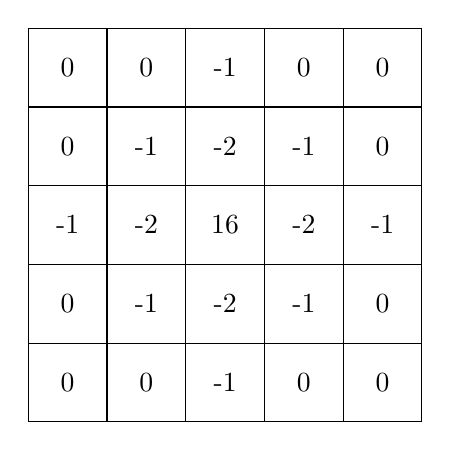
\begin{tikzpicture}

\foreach \x in {0,...,5} {
	\draw (\x,0) -- (\x,5);
	\draw (0,\x) -- (5,\x);
}

\foreach \x/\y in {0/0,1/0,0/1,3/0,4/0,4/1,0/3,0/4,1/4,3/4,4/4,4/3} {
	\node at  (\x+0.5,\y+0.5) {0};
}
\foreach \x/\y in {2/0,0/2,4/2,2/4,1/1,1/3,3/1,3/3} {
	\node at  (\x+0.5,\y+0.5) {-1};
}
\foreach \x/\y in {2/1,1/2,2/3,3/2} {
	\node at  (\x+0.5,\y+0.5) {-2};
}

\node at (2.5,2.5) {16};

\end{tikzpicture}}
		\caption{5x5 mask approximation. The negative of this mask would be used in practice}
	\end{subfigure}
	\caption{Marr-Hildreth}
\end{figure}

\textbf{Summary of the Marr-Hildreth edge detection:}
\begin{enumerate}
\item Filter the input image with an $n x n$ Gaussian lowpass filter $G(x,y)=e^{-\frac{x^2+y^2}{2\sigma^2}}$
\item Compute the Laplacian of the image resulting from Step 1. $\nabla ^2[G(x,y) \star f(x,y)]$
\item Find the zero crossing of the image from Step 2.
\end{enumerate}
\textbf{Size of the discrete LoG filter}
Rule of thumb: nxn LoG filter should have the smallest odd integer n greater than or equal to $6\sigma$.\\
\textbf{How to find the zero crossings?}\\
A zero-crossing exists, if at least one opposing pixelpair has a sign difference.
\begin{figure}[!h]
	\centering
	\begin{tikzpicture}
		\matrix[3x3mask]{
			a & b & c \\%
			d & 0 & d \\%
			c & b & a \\%
		};
	\end{tikzpicture}
	\caption{Zero-Crossing: opposing pixel pairs}	
\end{figure}

\paragraph{LoG DoG}
The Laplacian of Gaussian (LoG) can be approximated using a difference of Gaussian (DoG) filter
\begin{align}
DoG(x,y)=\frac{1}{2\pi\sigma_1^2}e^{-\frac{x^2+y^2}{2\sigma_1^2}}-\frac{1}{2\pi\sigma_2^2}e^{-\frac{x^2+y^2}{2\sigma_2^2}}\notag\\
\sigma^2=\frac{\sigma_1^2\sigma_2^2}{\sigma_1^2-\sigma_2^2}ln\left[\frac{\sigma_1^2}{\sigma_2^2}\right]\label{EQsigma}
\end{align}
\begin{itemize}
\item To compare LoG and DoG filters, they must have the same zero crossing
\item This can be achieved by setting $\sigma$ of the LoG in equation (\ref{EQsigma})
\item amplitude will scale differently, both can be normalized, such that the amplitude at 0 is 1
\item The negative functions are usually shown
\item The LoG and the DoG filters can be implemented by 1 D convolutions (they are separable)
\end{itemize}

\paragraph{Canny edge detector\buchSeite{719}}
\begin{enumerate}
	\item Smooth the image with a Gaussian filter.
		\begin{align*}
			G(x,y)	&= e^{-\frac{x^2+y^2}{2\sigma^2}} \\
			f_s(x,y)&=G(x,y)\star f(x,y
		\end{align*}
	\item Compute the gradient magnitude and angle images (Sobel operators).
		\begin{align*}
			M(x,y) 		&= \sqrt{g_x^2+g_y^2} \\
			\alpha(x,y)	&= tan^{-1}\left[\frac{g_y}{g_x}\right]
		\end{align*}
	\item Apply nonmaxima suppression to the gradient image:
		Let $d_1, d_2, d_3$ and $d_4$ denote the four basic edge directions for a 3x3 region: horizontal, $-45^\circ$, vertical and $-45^\circ$. 
		We can formulate the following nonmaxima suppression scheme for a 3x3 region centered at every point $(x,y)$ in $\alpha(x,y)$:
		\begin{enumerate}
			\item Find the direction $d_k$ that is closest to $\alpha(x,y)$
			\item If the value of $M(x,y)$ is less than at least one of its two neighbors alog $d_k$, let $g_N(x,y) = 0$ (suppression); otherwise, let $g_N(x,y) = M(x,y)$
		\end{enumerate}
	\item Use double thresholding and connectivity analysis to detect and link edges:
		\begin{itemize}
			\item $T_H$ a high treshold. If the values are above $T_H$, they are almost certainly a true edges
				\[
					g_{NH}(x,y) = g_N(x,y) \geq T_H
				\]
			\item $T_L$ a low threshold. High enough that most of the noise if filtered out, but much lower (2-3 times lower) than $T_H$ resulting in edge points that are likely to be true edges, but might also contain erroneous edges
				\[
					g_{NL}(x,y) = g_N(x,y) \geq T_L \qquad g_{NL} = g_{NL}(x,y) - g_{NH}(x,y)
				\]
			\item Now in $g_{NH}(x,y)$ are the strong edge pixels, while in $g_{NL}(x,y)$ are the weak ones.
			\item A large $T_H$ leads to gaps in the edges, which now can be filled using weak pixels in $g_{NL}(x,y)$ that are 8-connected to valid edge pixels in $g_{NH}(x,y)$:
				\begin{enumerate}
					\item Locate the next unvisited edge pixel, $p$, in $g_{NH}(x,y)$
					\item Mark as valid edge pixels all the weak pixels in $g_{NL}(x,y)$ that are connected to $p$ using 8-connectivity.
					\item If all nonzero pixels in $g_{NH}(x,y)$ have been visited go to Step d. Else, return to step a.
					\item Set to zero all pixels in $g_{NL}(x,y)$ that were not marked as valid edge pixels.
				\end{enumerate}
		\end{itemize}
\end{enumerate}


\subsubsection{Edge linking and boundary detection\buchSeite{725}}
Three schemes to link edges:\\
\paragraph{Local processing\buchSeite{726}}
For every point at a location the gradient vector magnitude and angle are compared with the magnitude and angle of points in a neighborhood. If these are similar, they belong to the same boundary. This can be indicated by giving them the same color and/or gray value.\\
A much simpler scheme can be used if the linking follows certain directions and the maximum gap size is roughly known.\\

\begin{enumerate}
	\item Compute the gradient magnitude and angle arrays, $M(x,y)$ and $\alpha(x,y)$ of the input image, $f(x,y)$
	\item Form a binary image, $g$, whose value at any pair of coordinates $(x,y)$ is given by:
		\[
			g(x,y) = 
				\begin{cases}
					1 & \text{if } M(x,y) > T_M \text{ and } \alpha(x,y) = A \pm T_A\\
					0 & \text{otherwise}
				\end{cases}
		\]
		Where $T_M$ is a threshold, $A$ is a specified angle direction, and $\pm T_A$ defines a "band" of acceptable directions about $A$.
	\item Scan the rows of $g$ and fill (set to 1) all gaps (sets of 0s) in each row that do not exceed a specified length, $K$.
		Note that, by definition, a gap is bounded at both ends by one or more 1s. 
		The rows are precessed individiually, with no memory between them.
	\item To detect gaps in any other direction, $\theta$, rotate $g$ by this angle and apply the horizontal scanning process procedure in Step 3.
		Rotate the result back by $-\theta$.
\end{enumerate}


\paragraph{Regional processing\buchSeite{728}}

If the location of a boundary is roughly known, it is possible to use the detected edge points as indicators for the suspected boundary.
\begin{enumerate}
\item Let P be a sequence of ordered, destinct, 1-valued points of a binary image. Specify two starting points, A and B. these are two starting vertices of the polygon.
\item Specify a threshold T, and two empty stacks, OPEN and CLOSED.
\item If the points in P correspond to a closed curve, put A into OPEN and put B into OPEN and CLOSED.
\item Compute the parameters of the line passing from the last vertex in CLOSED to the last vertex in OPEN.
\item Compute the distances from the line in Step 4 to all the points in P whose sequence places them between the vertices from Step 4. Select the point, $V_{max}$, with the maximum distance $D_{max}$ (ties are resolved arbitrarily)
\item If $D_{max}$, place $V_{max}$ at the end of the OPEN stack as a new vertex. Go to Step 4.
\item Else, remove the last vertex from Open and insert it as the last vertex of CLOSED.
\item If OPEN is not empty, go to Step 4.
\item Else, exit. The vertices in CLOSED are the vertices of the polygonal fit to the points in P.
\end{enumerate}
\begin{figure}[h]
	\centering
	\adjustbox{scale=0.5}{\usetikzlibrary{calc}
\begin{tikzpicture}[dot/.style={circle,inner sep=1pt, fill, name=#1}]

\begin{scope}[shift={(-5.5,1)}]
\node [dot=A] at (-2,-1.4) {};
\node [dot=B] at (-2.4,0.4) {};
\node [dot=C] at (1.2,-2.2) {};
\node [dot=D] at (2.2,-1.4) {};
\node [dot=E] at (2.6,-0.2) {};
\node [dot=F] at (2.4,0.8) {};
\node [dot=G] at (-1.6,1.8) {};
\node [dot=H] at (-2.2,1.2) {};
\node [dot=I] at (-2.4,-0.6) {};
\node [dot=J] at (2,1.6) {};
\node [dot=K] at (1.2,2) {};
\node [dot=L] at (0.4,2.4) {};
\node [dot=M] at (-0.8,2.2) {};
\draw[thick] (A) -- (C);
\draw[thick, dashed] ($(A)!(L)!(C)$) -- (L);
\end{scope}

\begin{scope}[shift={(0.9,1)}]
\node [dot=A] at (-2,-1.4) {};
\node [dot=B] at (-2.4,0.4) {};
\node [dot=C] at (1.2,-2.2) {};
\node [dot=D] at (2.2,-1.4) {};
\node [dot=E] at (2.6,-0.2) {};
\node [dot=F] at (2.4,0.8) {};
\node [dot=G] at (-1.6,1.8) {};
\node [dot=H] at (-2.2,1.2) {};
\node [dot=I] at (-2.4,-0.6) {};
\node [dot=J] at (2,1.6) {};
\node [dot=K] at (1.2,2) {};
\node [dot=L] at (0.4,2.4) {};
\node [dot=M] at (-0.8,2.2) {};
\draw[thick] (A) -- (L) -- (C);
\draw[thick, dashed] ($(A)!(H)!(L)$) -- (H);
\draw[thick, dashed] ($(L)!(F)!(C)$) -- (F);
\end{scope}

\begin{scope}[shift={(-5.5,-5)}]
\node [dot=A] at (-2,-1.4) {};
\node [dot=B] at (-2.4,0.4) {};
\node [dot=C] at (1.2,-2.2) {};
\node [dot=D] at (2.2,-1.4) {};
\node [dot=E] at (2.6,-0.2) {};
\node [dot=F] at (2.4,0.8) {};
\node [dot=G] at (-1.6,1.8) {};
\node [dot=H] at (-2.2,1.2) {};
\node [dot=I] at (-2.4,-0.6) {};
\node [dot=J] at (2,1.6) {};
\node [dot=K] at (1.2,2) {};
\node [dot=L] at (0.4,2.4) {};
\node [dot=M] at (-0.8,2.2) {};
\draw[thick] (A) -- (H) -- (L) -- (F) -- (C);
\draw[thick, dashed] ($(A)!(I)!(H)$) -- (I);
\draw[thick, dashed] ($(L)!(M)!(H)$) -- (M);
\draw[thick, dashed] ($(L)!(J)!(F)$) -- (J);
\draw[thick, dashed] ($(F)!(D)!(C)$) -- (D);
\end{scope}

\begin{scope}[shift={(0.9,-5)}]
\node [dot=A] at (-2,-1.4) {};
\node [dot=B] at (-2.4,0.4) {};
\node [dot=C] at (1.2,-2.2) {};
\node [dot=D] at (2.2,-1.4) {};
\node [dot=E] at (2.6,-0.2) {};
\node [dot=F] at (2.4,0.8) {};
\node [dot=G] at (-1.6,1.8) {};
\node [dot=H] at (-2.2,1.2) {};
\node [dot=I] at (-2.4,-0.6) {};
\node [dot=J] at (2,1.6) {};
\node [dot=K] at (1.2,2) {};
\node [dot=L] at (0.4,2.4) {};
\node [dot=M] at (-0.8,2.2) {};
\draw[thick] (A) -- (I) -- (H) -- (M) -- (L) -- (J) -- (F)-- (D) -- (C);
\end{scope}

\end{tikzpicture}}
	\caption{Regional Processing}
\end{figure}
\paragraph{Global processing using the Hough transform\buchSeite{733}}
\begin{figure}[h]
	\centering
	\begin{subfigure}{0.3\textwidth}
		\begin{tikzpicture}
	% Koordinatensystem
	\draw[->] (0,0) -- +(3,0) node[right] {$y$};
	\draw[->] (0,0) -- +(0,-3) node[below] {$x$};
	
	% Zwei Punkte definieren, anschreiben
	\coordinate (p1) at (1, -2.2);
	\coordinate (p2) at (2, -1.4);	
	\node[below right] at (p1) {$(x_i, y_i)$};
	\node[below right] at (p2) {$(x_j, y_j)$};
	\filldraw[black] (p1) circle (1pt)
					(p2) circle (1pt);
	
	% Linie zwischen Punkten
	\draw[thick, shorten <=-1cm, shorten >=-1cm] (p1) -- (p2);	
	% Mittelsenkrechte
	\draw ($ (p1)!(0,0)!(p2)$) -- (0,0) node[midway, above right] {$\rho$};
	
	% Winkel kennzeichnen
	\draw[->] (0,-1) arc (-90:-52:1);
	\node at  (0.3, -1.2) {$\theta$};
\end{tikzpicture}
		\caption{$xy$-plane}
	\end{subfigure}
	\begin{subfigure}{0.3\textwidth}
		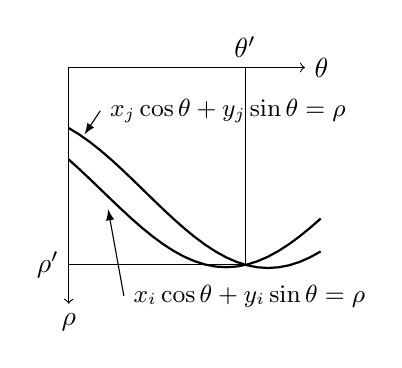
\begin{tikzpicture}[domain=0:3.2]
	% Koordinatensystem
	\draw[->] (0,0) -- +(3,0) node[right] {$\theta$};
	\draw[->] (0,0) -- +(0,-3) node[below] {$\rho$};
	% Kurven + Beschriftung
	% Die Kurven müssen etwas zurechtgestaucht werden, damit auch alles richtig passt. Ansosnten enprechen sie der richtigen Transfromation.
	\draw[thick] plot(\x, { -(3.14/2) + 0.4*(2.2 *cos( (\x + (3.14/2) ) r) + sin( (\x + (3.14/2) ) r)) });
	\draw[thick] plot(\x, { -(3.14/2) + 0.4*(1.4 *cos( (\x + (3.14/2) ) r) + 2* sin( (\x + (3.14/2) ) r)) });
	\draw[latex-] (0.2,-0.85) -- +(0.2,0.3) node[right] {\small $x_j\cos\theta + y_j\sin\theta = \rho$} ;
	\draw[latex-] (0.5,-1.8) -- +(0.2,-1.1) node[right] {\small $x_i\cos\theta + y_i\sin\theta = \rho$} ;
	% Schnittpunk der Geraden mit Beschriftung
	\draw (2.24,0) -- ++(0,-2.5) -- +(-2.24,0);
	\node[above] at (2.24, 0) {$\theta'$};
	\node[left] at (0, -2.5) {$\rho'$};
\end{tikzpicture}
		\caption{$\rho\theta$-plane}
	\end{subfigure}
	\begin{subfigure}{0.3\textwidth}
		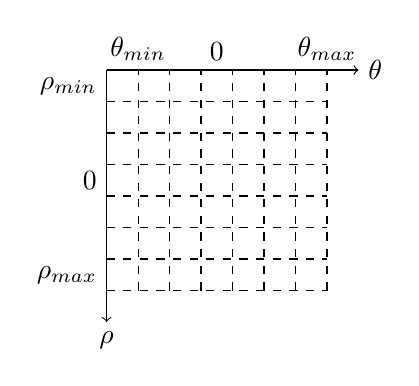
\begin{tikzpicture}
	% Koordinatensystem
	\draw[->] (0,3.2) -- +(3.2,0) node[right] {$\theta$};
	\draw[->] (0,3.2) -- +(0,-3.2) node[below] {$\rho$};
	\draw[step=0.4, dashed] (0,0.4) grid (2.8,3.2);
	\node[left] at (0,0.6) {$\rho_{max}$};
	\node[left] at (0,1.8) {$0$};
	\node[left] at (0,3) {$\rho_{min}$};
	\node[above] at (0.4,3.2) {$\theta_{min}$};
	\node[above] at (1.4,3.2) {$0$};
	\node[above] at (2.8,3.2) {$\theta_{max}$};
\end{tikzpicture}
		\caption{Accumulator Cells}
	\end{subfigure}
	\caption{Hough-Transform: From $xy$-plane to $\rho\theta$-plane}
\end{figure}
\begin{itemize}
\item Each point in the xy plane belongs to infinetly many lines $y_i=ax_i+b$
\item If we interpret this line equation differently, then $b=-x_ia+y_i$ represent for each point in the xy plane a line in the ab plane
\item For each point in the xy plane, a line can be drawn in the ab plane and the principal lines in the xy plane can be found by the points with the most intersections in the ab plane
\item Vertical lines require an infinite a, this does not work. Use the line normal as representation. A point in the xy plane does not result in a simple straight line in the parameter space ($\theta\rho$). The curve $\rho = f(\theta)$ is now a sinusoidal
\item Practical scheme
\begin{itemize}
\item For every $\theta_q$ in the $\rho\theta$ plane
\item Calculate $\rho = f(\theta)$ and quantize it into $\rho_q$
\item Increase the cell in the $\rho\theta$ plane at location ($\rho_q, \theta_q$) by one
\item end
\end{itemize}
\end{itemize}

\subsection{Thresholding\buchSeite{738}}
\subsubsection{Fundation\buchSeite{738}}
\begin{flalign}
& \text{single thresholding} && g(x,y)=\begin{cases}1 \qquad \text{if } f(x,y) > T \\0 \qquad  \text{if } f(x,y) \leq T \end{cases} &&\label{thresholdingBasic}\\
& \text{multiple thresholding} && g(x,y)=\begin{cases}a \qquad \text{if } f(x,y) > T_2 \\b \qquad  \text{if } T_1 < f(x,y)  \leq T_2 \\b \qquad  \text{if } f(x,y) \leq T_1 \end{cases} &&\label{thresholdingMultiple}
\end{flalign}

\subsubsection{Basic global thresholding\buchSeite{741}}

\begin{enumerate}
\item Select an initial estimate for the global threshold, T
\item Segment the image using T in Gleichung(\ref{thresholdingBasic}). This will produce two groups of pixels: $G_1$ consisting of all pixels with intensity values $> T$, and $G_2$ consisting of pixels with values $\leq T$
\item Compute the average (mean) intensity values $m_1$ and $m_2$ for the pixels in $G_1$ and $G_2$, repsectively
\item Compute a new threshold value: \begin{equation}
T=\frac{1}{2}(m_1+m_2)\notag
\end{equation} 
\item Repeat Steps 2 through 4 until the difference betwenn values of $T$ in successive iterations is smaller than a predefined paramter $\Delta T$
\end{enumerate}


\subsubsection{Optimum global thresholding using Otsu’s Method\buchSeite{742}}
Two different variances are important
\begin{itemize}
\item Within-class variance
\item Between-class variance
\end{itemize}

\begin{flalign*}
&\sigma_W^2 = P_1\sigma_1^2+P_2\sigma_2^2 
& & \sigma_W^2: \text{ Within-class variance}  && \\
&\sigma_B^2 = P_1(m_1-m_G)^2+P_2(m_2-m_G)^2
& & \sigma_B^2: \text{ Between-class variance}  && \\
&\sum_{i=0}^{L-1} p_i = 1 
& &  && \\
& m_G=\sum_{i=0}^{L-1} i \ p_i 
& & m_G: \text{ global mean}   && \\
&\sigma_G^2 = \sum_{i=0}^{L-1} (i-m_G)^2 p_i
& & \sigma_G^2: \text{global variance}  && \\
& P_1(k) =\sum_{i=0}^{k} p_i
& &  P_1: \text{ probability of the background}    && \\
& P_2(k)=\sum_{i=k+1}^{L-1}1-P_1(k)
& & P_2: \text{ probability of the object}  && \\
& m_1(k)=\frac{1}{P_1(k)}\sum_{i=0}^{k} i \ p_i
& &  m_1: \text{ mean intensity of the background}   && \\
& m_2(k)=\frac{1}{P_2(k)}\sum_{i=k+1}^{L-1} i \ p_i 
& &  m_2: \text{ mean intensity of the object}   && \\
& \sigma_B^2 = P_1(m_1-m_G)^2+P_2(m_2-m_G)^2 & &  \text{Using algebra to change the form}  && \\
&=P_1 P_2 (m_1-m_2)^2 = \frac{(m_G P_1 - m)^2}{P_1(1-P_1)} & &  && \\
&\sigma_B^2(k^*)=\max\limits_{0\leq k \leq L-1} \sigma_B^2(k)
& & \text{Optimum of k for maximizing is } k^*  && \\
&\eta(k)=\frac{\sigma_B^2(k)}{\sigma_G^2}
& & 0 \leq  \eta(k^*)\leq 1 
\end{flalign*}

\textbf{What to do now???}
\begin{enumerate}
	\item Compute the normalized histogram of the input image.
		Denote the components of the histogram by $p_i$, $i = 0, 1, 2, \ldots, L-1$
	\item Compute the cumulative sums, $P_1(k)$, for $k = 0, 1, 2, \ldots, L-1$, using Eq. 10.3-4 (welche das auch immer ist...).
	\item Compute the cumulative means, $m(k)$, for $k = 0, 1, 2, \ldots, L-1$, using Eq. 10.3-8 (jawohl, die musst du jetzt suchen!)
	\item Compute the global intensity mean, $m_g$, using Eq. 10.3-9
	\item Compute the between-class variance, $\sigma_B^2(k)$, for $k = 0, 1, 2, \ldots, L-1$, using Eq. 10.3-17
	\item Obtain the Otsu threshold, $k^\ast$, as the value $k$ for which $\sigma_B^2(k)$ is maximum.
		If the maximum is not unique, obtain $k^\ast$ by averaging the values of $k$ corresponding to the various maxima detected.
	\item Obtain the separability measure, $\eta^\ast$, by evaluating Eq. 10.3-16 at $k = k^\ast$.
\end{enumerate}

\subsubsection{Using Image Smoothing to Improve Global Thresholding\buchSeite{747}}
The obvious approach to improve the situation is to low pass filter the image, i.e., to smooth the image before the global thresholding method is applied
\subsubsection{Using Edges to Improve Global Thresholding\buchSeite{749}}
Only the strongest edges are usually kept, say the top 10\%
\subsubsection{Multiple Thresholds}

\begin{flalign*}
&\sigma_B^2 = P_1(m_1-m_G)^2+P_2(m_2-m_G)^2+P_3(m_3-m_G)^2 &&\\
& P_1(k) =\sum_{i=0}^{k_1} p_i && m_1(k)=\frac{1}{P_1(k)}\sum_{i=0}^{k_1} i \ p_i &&\\
& P_2(k)=\sum_{i=k_1+1}^{k_2} p_i && m_2(k)=\frac{1}{P_2(k)}\sum_{i=k_1+1}^{k_2} i \ p_i &&\\
& P_3(k)=\sum_{i=k_2+1}^{L-1} p_1 && m_3(k)=\frac{1}{P_3(k)}\sum_{i=k_2+1}^{L-1} i \ p_i &&\\
& m_G = P_1m_1 + P_2m_2 + P_3m_3 && P_1+P_2+P_3=1 &&\\
&\sigma_B^2(k_1^*,k_2^*)=\max\limits_{0\leq k_1 \leq k_2 \leq L-1} \sigma_B^2(k_1,k_2)&&
\eta(k_1^*,k_2^*)=\frac{\sigma_B^2(k_1^*,k_2^*)}{\sigma_G^2}&&\\
\end{flalign*}
\subsubsection{Variable Thresholding\buchSeite{756}}
\paragraph{Image Partitioning\buchSeite{756}}
The simplest approach is to partition a given image into non overlapping regions and then use Otsu's method on smaller regions.\\
\paragraph{Based on local image properties\buchSeite{758}}
A threshold is computed for each point. The threshold depends on some property of a local neighborhood. Common properties are the mean and standard deviation for each pixel.
An even more powerful scheme can be built, if the 1 or 0 decision is based on some logical condition.\\
\subsubsection{Multivariable Thresholding\buchSeite{761}}
\subsection{Region based segmentation\buchSeite{763}}
The goal is to segment the image into regions directly, not using abrupt changes or thresholding.
\subsubsection{Region growing\buchSeite{763}}
\begin{enumerate}
\item Find all connected components in $S(x,y)$ and erode each connected component to one pixel; label all such pixels found as 1. All other pixels in S are labeled 0.
\item Form an image $f_Q$ such that, at a pair of coordinates $(x,y)$, let $f_Q(x,y)=1$ if the input image satisfies the given predicate, Q, at those coordinates; otherwise, let $f_Q(x,y)=0$
\item Let $g$ be an image formed by appending to each seed point in S all the 1-valued points in $f_Q$ that are 8-connected to that seed point
\item Label each connected component in $g$ with a different region label (e.g. 1,2,3,...). This is the segmented image optained by Region growing.
\end{enumerate}
\subsubsection{Region splitting and merging\buchSeite{766}}
The image is subdivided initially into a set of arbitrary disjoint regions and then the regions are merge and or split in an attempt to improve the segmentation.\\
A common scheme to split images is a quadtree.\\
\begin{enumerate}
	\item Split into four disjoint quadrants any region $R_i$ for wich $Q(R)= FALSE$. 
	\item When no further splitting is possible, merge any adjacent regions $R_i$ and $R_k$ for which $Q(R_j\bigcup R_k) = TRUE$.
	\item Stop when no further merging is possible
\end{enumerate}
\begin{figure}[h]
	\centering
	\begin{subfigure}{0.3\textwidth}
		\centering
		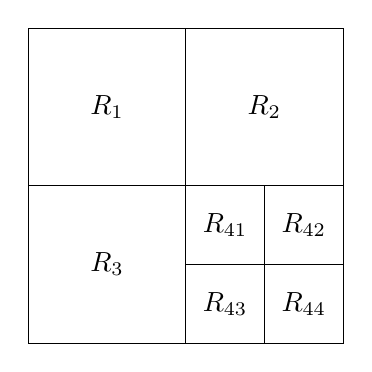
\begin{tikzpicture}[
	every node/.style={
		draw, 
		minimum width=2cm, 
		minimum height=2cm
	}]
	\node at (0,2) {$R_1$};
	\node at (2,2) {$R_2$};
	\node at (0,0) {$R_3$};
	\begin{scope}[
		xshift=1.5cm,
		yshift=-0.5cm,
		every node/.style={
			draw, 
			minimum width=1cm, 
			minimum height=1cm}
		]
		\node at (0,1) {$R_{41}$};
		\node at (1,1) {$R_{42}$};
		\node at (0,0) {$R_{43}$};
		\node at (1,0) {$R_{44}$};
	\end{scope}
	
\end{tikzpicture}
		\caption{Partioned image}
	\end{subfigure}
	\begin{subfigure}{0.5\textwidth}
		\centering
		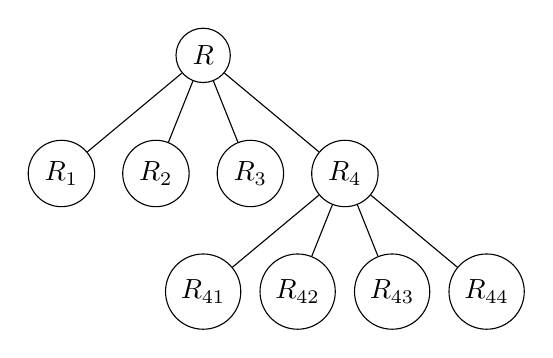
\begin{tikzpicture}[
	every node/.style={draw, circle},
	level 1/.style={sibling distance=12mm},
	level 2/.style={sibling distance=12mm},
	]
	\node {$R$}
		child { node {$R_1$}}
		child { node {$R_2$}}
		child { node {$R_3$}}
		child { node {$R_4$}
			child { node {$R_{41}$}}
			child { node {$R_{42}$}}
			child { node {$R_{43}$}}
			child { node {$R_{44}$}}
		};		
\end{tikzpicture}
		\caption{Corresponding quadtree. $R$ represents the entire image region.}
	\end{subfigure}
	\caption{Quadtree example}
\end{figure}


\subsection{Segmentation using morphological watersheds\buchSeite{769}}
\subsubsection{Background\buchSeite{769}}
The basic idea is to think of images as 3D landscapes. There are three kinds of points:
\begin{itemize}
\item Points belonging to a regional minimum.
\item Points, where water would flow. These are called catchment basin.
\item Points, where water would be equally likely to fall to more than one such minimum. These are called watershed.
\end{itemize}
Basic idea:
\begin{itemize}
\item In each basin a hole is punched
\item The topological image is pushed into a full bathtub. The water rises uniformly in the different basing
\item As soon as the water in different basins want to merge, a dam is build
\item At the end only the dams are left. These are the watershed lines wich are connected boundaries segmenting the image into different regions.
\end{itemize}
\subsubsection{Dam Construction\buchSeite{772}}
\begin{itemize}
\item The easiest way to construct such a dam is using dilation
\item When basins merge, then a dam needs to be constructed
\end{itemize}
\subsubsection{Watershed segmentation algorithm\buchSeite{774}}
\begin{itemize}
\item $T[n]$ is the set of coordinates flooded $T[n] = {(s,t)|g(s,t)<n}$
\item The flooding goes in integers from $n=min+1$ to $n=max+1$
\item The algorithm starts with $C[min+1]=T[min+1]$. This leads to $C_{min+1}(M_i)$ for every minimum. $C[n]=\bigcup\limits_{i=1}^{R}C_n(M_i)$
\item Now $C[n]$ is created from $C[n-1]$
\begin{enumerate}
\item Was a new basin discovered?
\item Did the basins simply expand?
\item Did two basins merge?
\end{enumerate}
%TODO Algorithm Seite 114 und 115
%TODO dam building algo Seite 112
\end{itemize}
\subsection{The use of motion in segmentation\buchSeite{778}}
\subsubsection{Spatial Techniques\buchSeite{778}}
\subsubsection{Frequency Domain Techniques\buchSeite{782}}
%TODO Seiten 117, 118, 119
%TODO Frequency Domain Techniques praktikum read, auch hinein nehmen
